
%(BEGIN_QUESTION)
% Copyright 2009, Tony R. Kuphaldt, released under the Creative Commons Attribution License (v 1.0)
% This means you may do almost anything with this work of mine, so long as you give me proper credit

Sketch connecting wires such that the relay will energize and turn on the lamp when the normally-open (NO) pushbutton switch is pressed.  Use the following schematic diagram as a guide:

$$\includegraphics[width=15.5cm]{i03835x01.eps}$$

Note how the relay coil and lamp are separate (parallel) branches in this circuit.  The pushbutton switch {\it only} carries coil current, while the relay's switch contact {\it only} carries lamp current.

\vskip 20pt \vbox{\hrule \hbox{\strut \vrule{} {\bf Suggestions for Socratic discussion} \vrule} \hrule}

\begin{itemize}
\item{} Suppose the battery is rated at 12 volts, the lamp has a ``hot'' filament resistance of 3.2 ohms, and the relay coil has a wire resistance of 240 ohms.  Calculate the amount of current carried by the switch when it is pressed.
\end{itemize}

\underbar{file i03835}
%(END_QUESTION)





%(BEGIN_ANSWER)

Bear in mind that this is not the {\it only} possible circuit solution:

$$\includegraphics[width=15.5cm]{i03835x02.eps}$$

Challenge yourself by designing a different circuit to meet the same criteria! 

%(END_ANSWER)





%(BEGIN_NOTES)

Note how a schematic diagram was provided for you, to help you determine where each and every wire should go.  In real-life situations, you may not be given any schematic diagram at all.  In such cases, it is an excellent problem-solving strategy to first sketch your own schematic diagram, before attempting to sketch a pictorial diagram or connect real wires to the devices.  The concept here is that schematic diagrams are much easier to interpret and understand than pictorial diagrams where wires tend to cross over each other more, and where components are not always optimally placed.

%INDEX% Pictorial circuit review (relay circuit)

%(END_NOTES)


